\begin{frame}

{species ARE related}

\begin{longtable}[c]{@{}cc@{}}
\toprule\addlinespace
Evolution & Ecology
\\\addlinespace
\midrule\endhead
Phylogeny & Food Web
\\\addlinespace
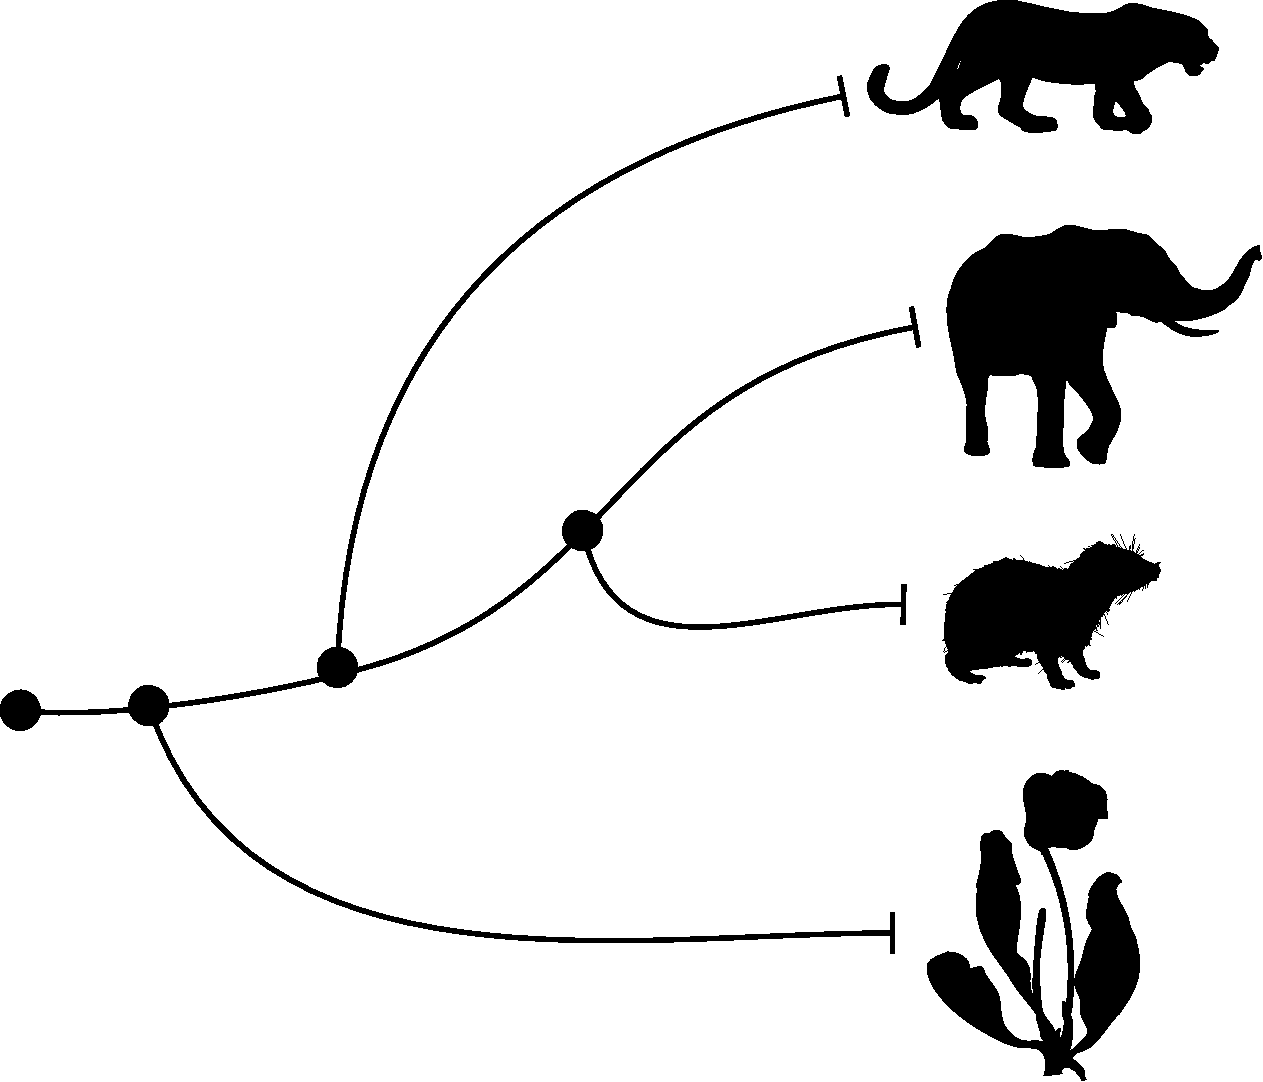
\includegraphics{images/small_phylo.pdf} &
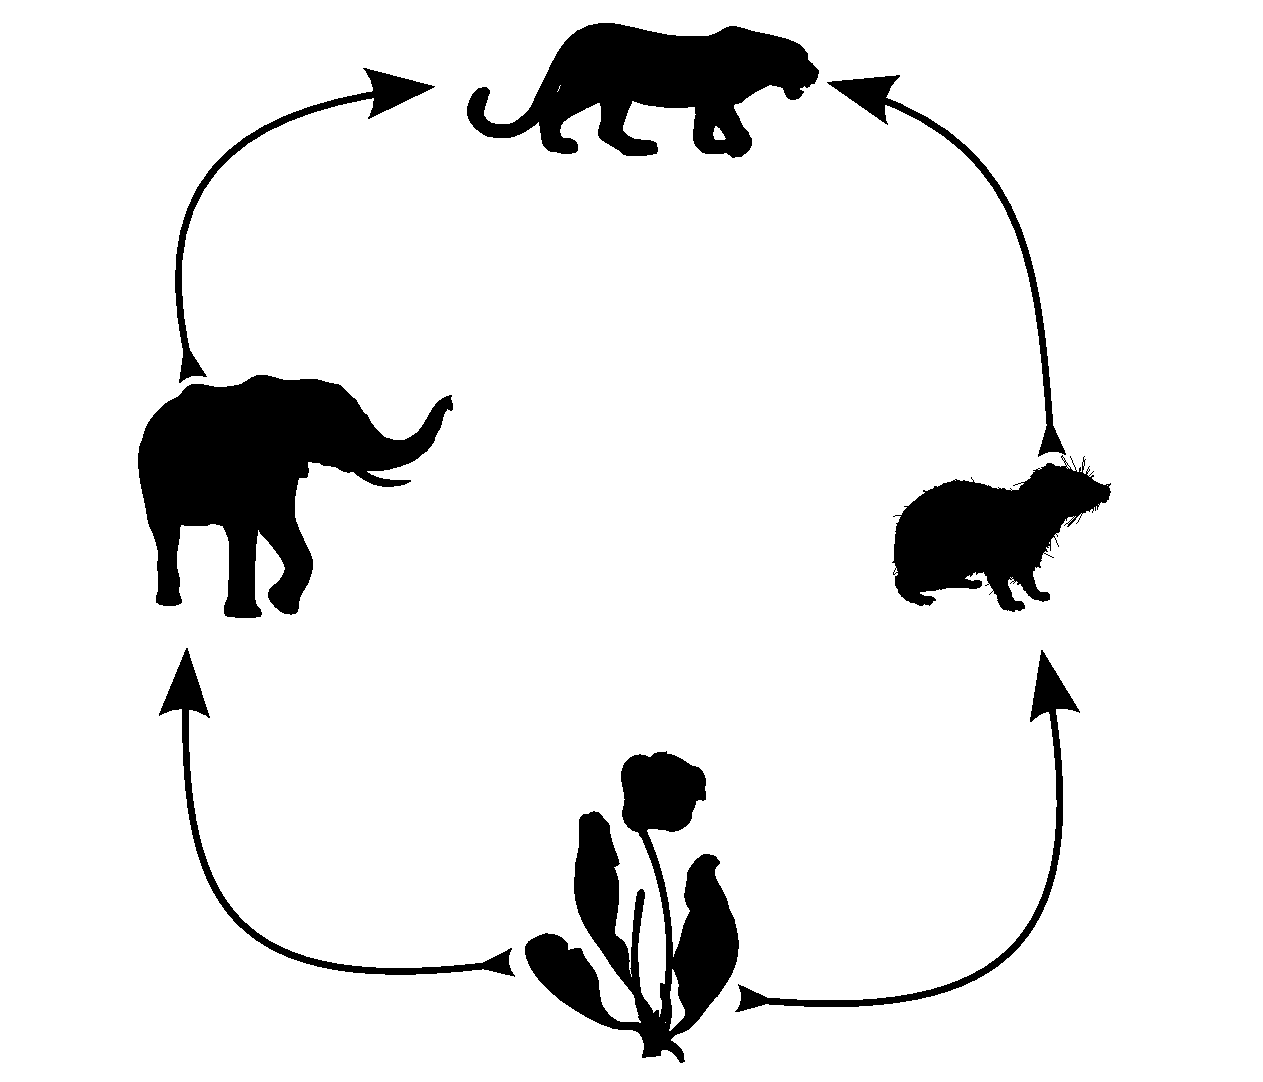
\includegraphics{images/small_fw.pdf}
\\\addlinespace
\bottomrule
\end{longtable}

{Evolution in/of Ecology}

Evolution shaped the stochastic backbones of Food Webs

{{[}Two images: Serengeti and Weddell{]}}

{Food Webs embedded}

\begin{itemize}[<+->]
\item
  Random Dot Product Graphs

  \begin{figure}[htbp]
  \centering
  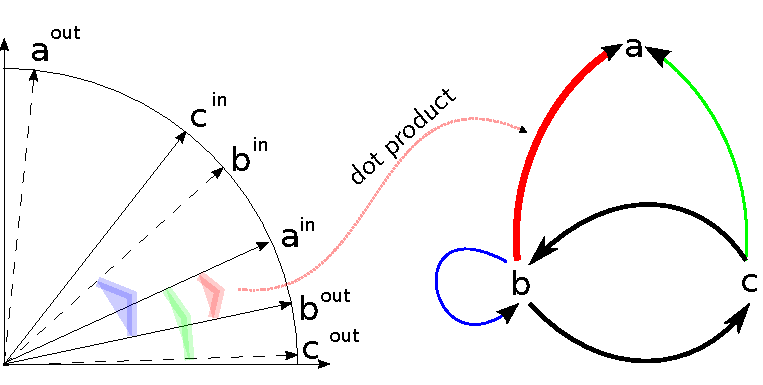
\includegraphics{images/RDPGmodel.pdf}
  \caption{image}
  \end{figure}
\item
  Phylogenetic vs.~Observed traits

  \[\textrm{vcv}\left( \hat{x} | \tau, \mbox{model} \right) \mbox{ vs. } \textrm{vcv}\left(x\right)\]
\end{itemize}

{More questions (than answers)}

\begin{itemize}[<+->]
\item
  There is phylogenetic signal\\{p-values anybody?}
\item
  It is quite weak\\{$20\% ~ 30\%$ of variation explained}
\item
  It saturates with
  dimensionality\\{$d \in \left\{2, \dots , 8 \right\}$}
\item
  $\therefore$ ``fine wirings'' may be deceiving
\item
  Evolutionary model is inadequate\\{no interaction effects}
\end{itemize}

{(Not a) Conclusion}

\begin{itemize}[<+->]
\item
  Spoiler 1: Evolutionary distinctiveness vs.~Web Centrality\\{Do
  evolutionary unique species play a keystone role in Food Webs?}
\item
  Spoiler 2: An ecological informed model of species evolution maybe
  it's (almost) there.\\{I am looking at you, Ornstein and Uhlenbecki
  $\dots$}
\end{itemize}

{Thanks!}

Joint work with Daniel B. Stouffer (University of Canterbury)

Many thanks to Mike Steel; Carey Priebe; A. Mooers', D.B. Stouffer's \&
J. Tylianakis's labs; \ldots{}

Funds by the Allan Wilson Centre for Molecular Ecology and Evolution.

\end{frame}
